%%%%%%%%%%%%%%%%%%%%%%%%%%%%% Define Article %%%%%%%%%%%%%%%%%%%%%%%%%%%%%%%%%%
\documentclass{article}
%%%%%%%%%%%%%%%%%%%%%%%%%%%%%%%%%%%%%%%%%%%%%%%%%%%%%%%%%%%%%%%%%%%%%%%%%%%%%%%

%%%%%%%%%%%%%%%%%%%%%%%%%%%%% Using Packages %%%%%%%%%%%%%%%%%%%%%%%%%%%%%%%%%%
\usepackage{geometry}
\usepackage{graphicx}
\usepackage{amssymb}
\usepackage{amsmath}
\usepackage{amsthm}
\usepackage{empheq}
\usepackage{mdframed}
\usepackage{booktabs}
\usepackage{lipsum}
\usepackage{graphicx}
\usepackage{color}
\usepackage{psfrag}
\usepackage{pgfplots}
\usepackage{babel}
\usepackage{hyperref}
\usepackage[scr]{rsfso}
\usepackage{thmtools}
\usepackage{theoremref}
\usepackage{floatrow}
\usepackage{bm}

%%%%%%%%%%%%%%%%%%%%%%%%%%%%%%%%%%%%%%%%%%%%%%%%%%%%%%%%%%%%%%%%%%%%%%%%%%%%%%%
%%%%%%%%%%%%%%%%%%%%%%%%%%%%% Package Setups %%%%%%%%%%%%%%%%%%%%%%%%%%%%%%%%%%
\graphicspath{ {./images/} }
\hypersetup{
    colorlinks,
    citecolor = black,
    filecolor = black,
    linkcolor = black,
    urlcolor = black
}
%%%%%%%%%%%%%%%%%%%%%%%%%%%%%%%%%%%%%%%%%%%%%%%%%%%%%%%%%%%%%%%%%%%%%%%%%%%%%%%
% Other Settings

%%%%%%%%%%%%%%%%%%%%%%%%%% Page Setting %%%%%%%%%%%%%%%%%%%%%%%%%%%%%%%%%%%%%%%
\geometry{letterpaper}

%%%%%%%%%%%%%%%%%%%%%%%%%% Define some useful colors %%%%%%%%%%%%%%%%%%%%%%%%%%
\definecolor{ocre}{RGB}{243,102,25}
\definecolor{mygray}{RGB}{243,243,244}
\definecolor{deepGreen}{RGB}{26,111,0}
\definecolor{shallowGreen}{RGB}{235,255,255}
\definecolor{deepBlue}{RGB}{61,124,222}
\definecolor{shallowBlue}{RGB}{235,249,255}
%%%%%%%%%%%%%%%%%%%%%%%%%%%%%%%%%%%%%%%%%%%%%%%%%%%%%%%%%%%%%%%%%%%%%%%%%%%%%%%

%%%%%%%%%%%%%%%%%%%%%%%%%% Define an orangebox command %%%%%%%%%%%%%%%%%%%%%%%%
\newcommand\orangebox[1]{\fcolorbox{ocre}{mygray}{\hspace{1em}#1\hspace{1em}}}
%%%%%%%%%%%%%%%%%%%%%%%%%%%%%%%%%%%%%%%%%%%%%%%%%%%%%%%%%%%%%%%%%%%%%%%%%%%%%%%

%%%%%%%%%%%%%%%%%%%%%%%%%%%% English Environments %%%%%%%%%%%%%%%%%%%%%%%%%%%%%
\newtheoremstyle{mytheoremstyle}{3pt}{3pt}{\normalfont}{0cm}{\rmfamily\bfseries}{}{1em}{{\color{black}\thmname{#1}~\thmnumber{#2}}\thmnote{\,--\,#3}}
\newtheoremstyle{myproblemstyle}{3pt}{3pt}{\normalfont}{0cm}{\rmfamily\bfseries}{}{1em}{{\color{black}\thmname{#1}~\thmnumber{#2}}\thmnote{\,--\,#3}}
\theoremstyle{mytheoremstyle}
\newmdtheoremenv[linewidth=1pt,backgroundcolor=shallowGreen,linecolor=deepGreen,leftmargin=0pt,innerleftmargin=20pt,innerrightmargin=20pt,]{theorem}{Theorem}[section]
\theoremstyle{mytheoremstyle}
\newmdtheoremenv[linewidth=1pt,backgroundcolor=shallowBlue,linecolor=deepBlue,leftmargin=0pt,innerleftmargin=20pt,innerrightmargin=20pt,]{definition}{Definition}[section]
\theoremstyle{myproblemstyle}
\newmdtheoremenv[linewidth=1pt,linecolor=black,leftmargin=0pt,innerleftmargin=10pt,innerrightmargin=10pt,]{problem}{Problem}[section]
\newtheoremstyle{break}{3pt}{3pt}{\normalfont}{}{\rmfamily\bfseries}{}{1em}{{\color{blue}\thmname{#1}~\thmnumber{#2}}\thmnote{\,--\,#3}}
\theoremstyle{break}
\newmdtheoremenv[linewidth=1pt, linecolor=blue,leftmargin=0pt,innerleftmargin=10pt,innerrightmargin=10pt]{solution}{Solution}[section]
\renewcommand{\listtheoremname}{List of Problems and Solutions}
\renewcommand*\contentsname{Table of Contents}
\newsavebox\foobox
\newlength{\foodim}
\newcommand{\Laplace}{\mathscr{L}}
\newcommand{\LaplaceInverse}{\mathscr{L}^{-1}}
%%%%%%%%%%%%%%%%%%%%%%%%%%%%%%%%%%%%%%%%%%%%%%%%%%%%%%%%%%%%%%%%%%%%%%%%%%%%%%%

%%%%%%%%%%%%%%%%%%%%%%%%%%%%%%% Plotting Settings %%%%%%%%%%%%%%%%%%%%%%%%%%%%%
\usepgfplotslibrary{colorbrewer}
\pgfplotsset{width=8cm,compat=1.9}
%%%%%%%%%%%%%%%%%%%%%%%%%%%%%%%%%%%%%%%%%%%%%%%%%%%%%%%%%%%%%%%%%%%%%%%%%%%%%%%

%%%%%%%%%%%%%%%%%%%%%%%%%%%%%%% Title & Author %%%%%%%%%%%%%%%%%%%%%%%%%%%%%%%%
\title{Intro to Control Systems Final Notes}
\author{Akhil Chawathe}
%%%%%%%%%%%%%%%%%%%%%%%%%%%%%%%%%%%%%%%%%%%%%%%%%%%%%%%%%%%%%%%%%%%%%%%%%%%%%%%


%%%%%%%%%%%%%%%%%%%%%%%%%%%%%%% Document %%%%%%%%%%%%%%%%%%%%%%%%%%%%%%%%%%%%%%
\begin{document}

\maketitle

%%%%%%%%%%%%%%%%%%%%%%%%%%%%%%% Abstract %%%%%%%%%%%%%%%%%%%%%%%%%%%%%%%%%%%%%%
\begin{abstract}
	This document aims to provide a comprehensive summary of the course ELG 3155.
	The summaries will attempt to abstain from any complex language that may
	confuse the reader or overcomplicate a simple explanation.
	The next natural question is, why not make this handwritten?
	The answer is simple: the document is intended to be easily searchable and
	accessible by any student who may need it, either now, or in the future.
	This document will not numerically correspond to the textbook nor the lecture
	notes as that may change from year to year, instead,
	it will have its own easy to follow structure.
	The document is divided into sections, each corresponding to a
	topic covered in the course.
	The detailed list of the topics covered are:

	\begin{enumerate}
		\item Review of Signals and Systems (This will only have the stuff that matters for this course)
		\item Transfer Functions of:
		      \subitem Electrical Systems
		      \subitem Mechanical Systems
		      \subitem Rotational Mechanical Systems
		\item State Space
		      \subitem Analysis of:
		      \subsubitem Electrical Systems
		      \subsubitem Mechanical Systems
		      \subsubitem Rotational Mechanical Systems
		      \subitem Converting Transfer Functions to State Space
		      \subitem Converting State Space to Transfer Functions
		\item System Response
		      \subitem Poles and Zeros
		      \subitem First Order Systems
		      \subitem Transient Response
		      \subitem Second Order Systems
		      \subsubitem Response Types of Second Order Systems
		      \subsubitem General Analysis of Second Order Systems
		      \subsubitem Damping Ratios
		\item Reduction of Multiple Subsystems
		      \subitem Open Loop Systems
		      \subitem Closed Loop Systems
		      \subitem Block Diagrams
		      \subitem Forms of Block Diagrams
		      \subitem Reduction of Block Diagrams
		      \subitem Signal Flow Graphs and Mason's Rule
		      \subitem Reduction of Signal Flow Graphs
		\item Alternatives State Space Representations
		\item Stability
		      \subitem Poles of an Unstable LTI System
		      \subitem Routh-Hurwitz Criterion
		      \subsubitem Routh Tables
		      \subsubitem Special Cases
		      \subitem Stability of State Space Systems
		\item Steady State Errors
		      \subitem Typed of Inputs:
		      \subsubitem Step Inputs
		      \subsubitem Ramp Inputs
		      \subsubitem Parabolic Inputs
		      \subitem System Errors
		      \subitem Final Value Theorem
		      \subitem Error Constants
		      \subitem System Types
		\item Root Locus
		      \subitem Properties of Root Locus
		      \subitem Sketching Root Locus
		      \subitem Real Axis Intersections and Break-In/Breakaway Points
		      \subitem $j\omega$ Axis Intersections
		      \subitem Angles of Departure and Arrival
		      \subitem Transient Response Via Gain Adjustment
		      \subitem Second Order Approximations
		\item Design Via Root Locus
		      \subitem Reducing Errors
		      \subitem Improving Transient Response
		      \subitem Improving Steady State Errors
		      \subitem Proportional-Plus-Integral Controllers
		      \subitem Phase Lag Compensation
		      \subitem Cascade Compensation
		      \subitem Proportional-Plus-Derivative Controllers
		      \subitem Phase Lead Compensation
		      \subitem PID Compensation
		      \subitem Phase Lag-Lead Compensation
	\end{enumerate}
\end{abstract}

%%%%%%%%%%%%%%%%%%%%%%%%%%% Table of Contents %%%%%%%%%%%%%%%%%%%%%%%%%%%%%%%

\newpage
\tableofcontents
\newpage
\listoffigures
\newpage
\listoftheorems[ignoreall, show = {problem,solution},swapnumber]{}
\newpage

%%%%%%%%%%%%%%%%%%%%%%%%%%% Start of the Document %%%%%%%%%%%%%%%%%%%%%%%%%%%%%%%

%%%%%%%%%%%%%%%%%%%%%%%%%%% Section 1 %%%%%%%%%%%%%%%%%%%%%%%%%%%%%%%   
\section{Review of Signals and Systems}
TODO: Add Material as needed from the course notes

\subsection{The Laplace Transform}

The Laplace Transform is a powerful tool used to analyze signals and systems.
It is defined as:
\begin{equation}
	F(s) = \mathcal{L}\{f(t)\} = \int_0^\infty f(t)e^{-st}dt
\end{equation}
Where $s = \sigma + j\omega$ is a complex number.
The inverse Laplace Transform is defined as:
\begin{equation}
	f(t) = \mathcal{L}^{-1}\{F(s)\} = \frac{1}{2\pi j} \int_{\sigma-j\infty}^{\sigma+j\infty} F(s)e^{st}ds = f(t) u(t)
\end{equation}
Where $u(t)$ is the unit step function, defined as:
\begin{equation}
	u(t) = \begin{cases}
		1 & t \geq 0 \\
		0 & t < 0
	\end{cases}
\end{equation}
Realistically, we don't need to know the definition, as other people have done the hard work for us, and we can use tables to find the Laplace Transform of a function.
The following table shows some common Laplace Transforms found in this course:
\begin{figure}[h]
	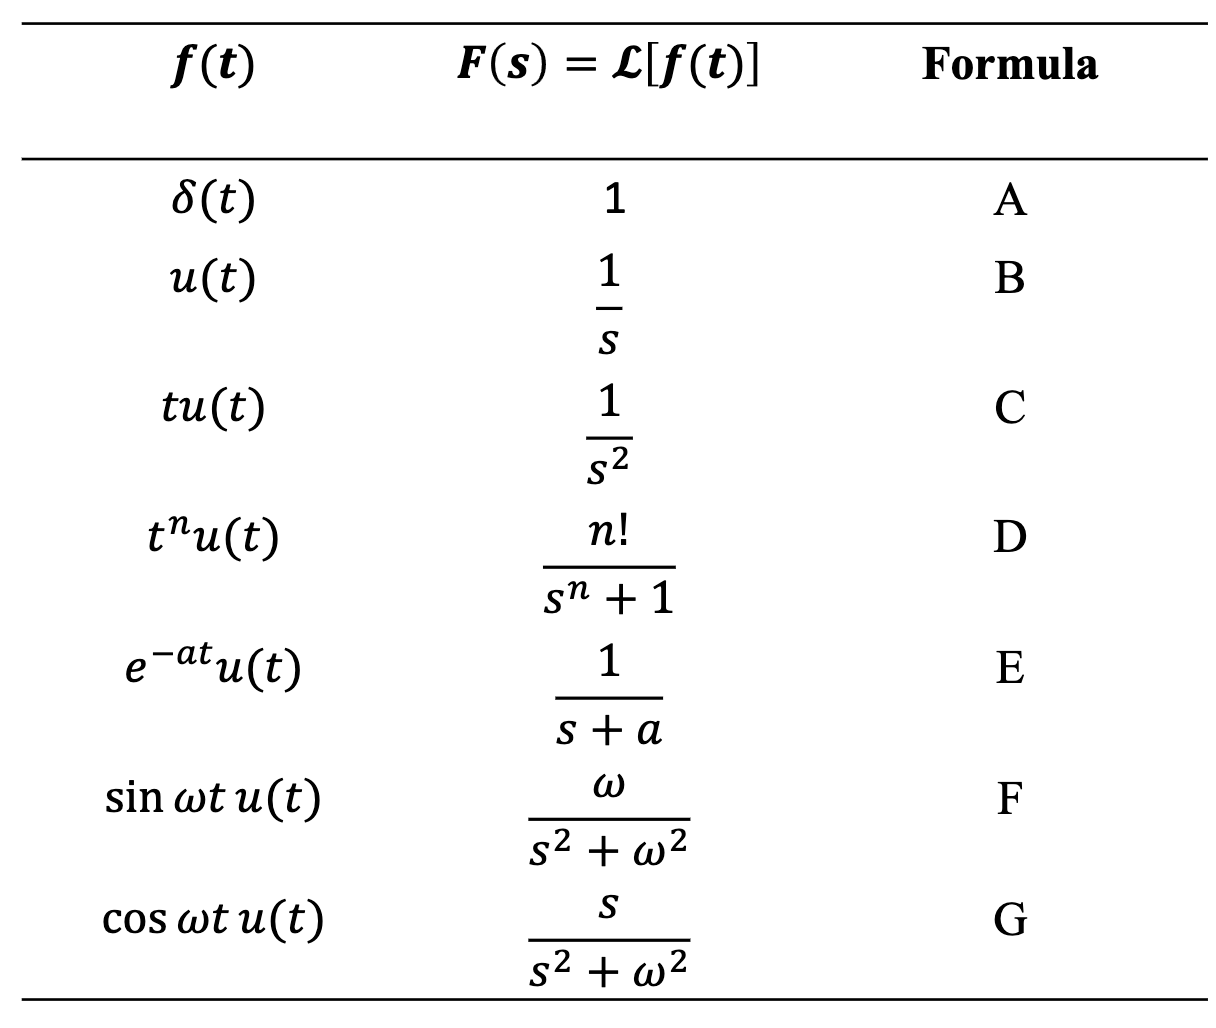
\includegraphics[scale=0.2]{Laplace Transforms Table}
	\centering
	\caption{Common Laplace Transforms}
\end{figure}
\newpage
Sometimes, we may need to find the Laplace Transform of some function $f(t)$ that is not in the table. To do this, we can use the following properties of the Laplace Transform:

\begin{figure}[h]
	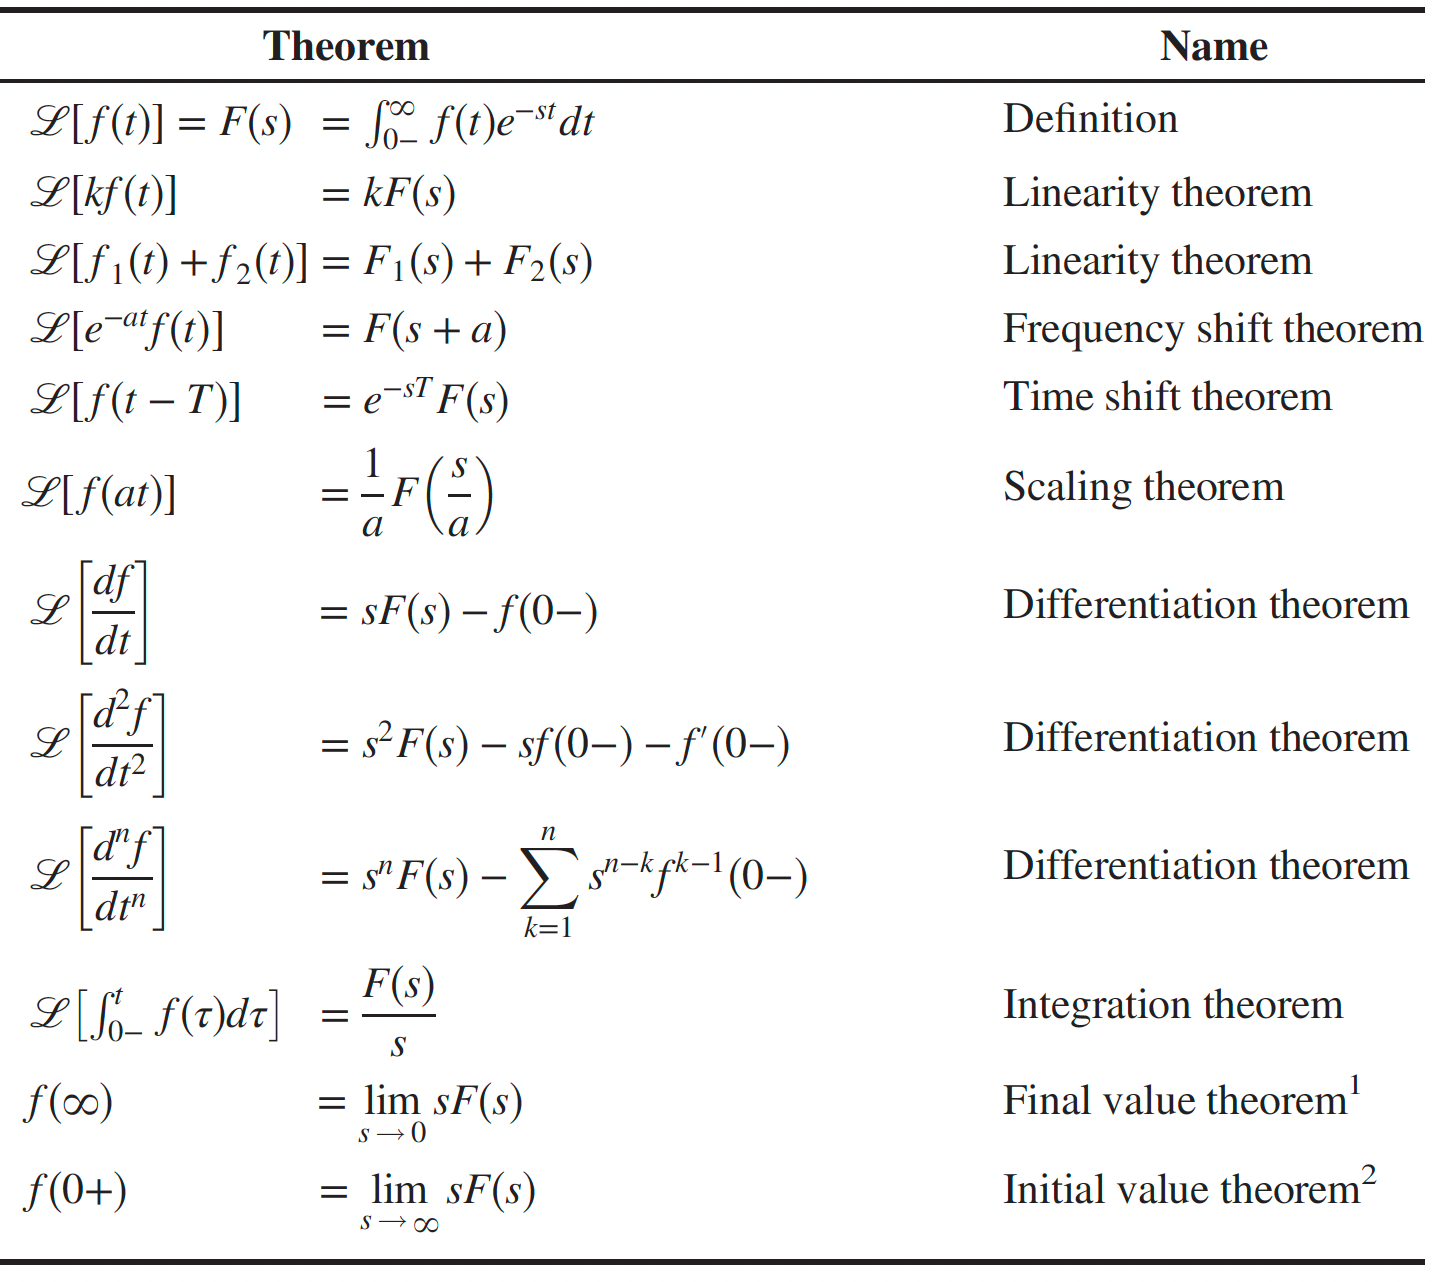
\includegraphics[scale=0.2]{Laplace Transform Properties}
	\centering
	\caption{Properties of the Laplace Transform}
\end{figure}
%%%%%%%%%%%%%%%%%%%%%%%%%%% Subsection 1.2 %%%%%%%%%%%%%%%%%%%%%%%%%%%%%%% 
\subsection{Partial Fraction Expansion}
Partial Fraction Expansion is a method used to simplify a complex rational function into a sum of simpler fractions. The general form of a rational function is:
\begin{equation}
	F(s) = \frac{Y(s)}{X(s)}
\end{equation}

Where $Y(s)$ and $X(s)$ are polynomials in $s$. The goal is to simplify $F(s)$ into a sum of simpler fractions. The general form of the simpler fractions is:
\begin{equation}
	F(s) = \frac{K_1}{s-p_1} + \frac{K_2}{s-p_2} + \ldots + \frac{K_n}{s-p_n}
\end{equation}

Where $K_i$ and $p_i$ are constants. For partial fraction expansion to work, the degree of $Y(s)$ must be less than the degree of $X(s)$. There are three cases you will encounter when performing partial fraction expansion:

\begin{enumerate}
	\item Distinct Real Roots
	\item Repeated Real Roots
	\item Complex Roots
\end{enumerate}
Normally, you would use the following steps to perform partial fraction expansion:
\begin{enumerate}
	\item Factorize the denominator of $F(s)$
	\item Write $F(s)$ in the form of equation (4)
	\item Multiply both sides by $X(s)$
	\item Solve for the constants $K_i$ and $p_i$
\end{enumerate}

But, that is a lengthy process. Instead, there are some tricks you can use to make the process easier. Let's do this on a case-by-case basis. There will be sections outlining each case and how to solve it.

\subsubsection{Distinct Real Roots}
When the denominator of $F(s)$ can be factored relatively easily or is comprised of roots that can be found via the quadratic formula, and the roots are different from each other as well as real (meaning they are not imaginary numbers nor complex numbers), the partial fraction expansion will look like this:
\begin{equation}
	\frac{Y(s)}{X(s)} = \frac{Y(s)}{(s-p_1)(s-p_2) \ldots (s-p_n)} = \frac{K_1}{s-p_1} + \frac{K_2}{s-p_2} + \ldots + \frac{K_n}{s-p_n}
\end{equation}

To solve this, you would use the following steps, bear in mind, this is a shortcut, and you can use the general steps if you want to:
\begin{enumerate}
	\item Factor the denominator of $F(s)$
	\item Separate the terms on the right side of the equation into separate fractions. Each fraction will have a constant $K_i$ and a root $p_i$. This is the same as equation (6).
	\item Create a limit of the rest of the equation $s$ approaches $p_i$. This will give you an equation with $K_i$ on one side and the limit on the other side. The equation with the limit you are evaluating will not have the term with $p_i$ in it.
	\item Solve for $K_i$.
	\item Repeat for all roots.
\end{enumerate}

If you are not clear on how to do this, you may be able to get a better understanding by looking at the following example:
%%%%%%%%%%%%%%%%%%%%%%%%%%% Subsection 1.2.1 %%%%%%%%%%%%%%%%%%%%%%%%%%%%%%% 
\begin{problem}[Distinct Real Roots]
Find the partial fraction expansion of the following function:
\begin{equation}
	F(s) = \frac{32}{s(s^2 + 12s + 32)}
\end{equation}
\end{problem}
Let's walk through this problem using the steps I outlined above:
\begin{solution}[\textcolor{blue}{Distinct Real Roots}]~
	\begin{enumerate}
		\item Factor the denominator of $F(s)$:
		      \begin{equation}
			      F(s) = \frac{32}{s(s^2 + 12s + 32)} = \frac{1}{s(s+4)(s+8)}
		      \end{equation}
		\item Separate the terms on the right side of the equation into separate fractions. Each fraction will have a constant $K_i$ and a root $p_i$. This is the same as equation (6):
		      \begin{equation}
			      F(s) = \frac{32}{s(s+4)(s+8)} = \frac{K_1}{s} + \frac{K_2}{s+4} + \frac{K_3}{s+8}
		      \end{equation}
		\item Create a limit of the rest of the equation $s$ approaches $p_i$. This will give you an equation with $K_i$ on one side and the limit on the other side. The equation with the limit you are evaluating will not have the term with $p_i$ in it. We will also solve for $K_1$ in this step:
		      \begin{equation}
			      K_1 = \frac{32}{(s+4)(s+8)} \Big|_{s \to 0} = \frac{32}{(4)(8)} = 1
		      \end{equation}
		\item Repeat for all roots:
		      \subitem Solving for $K_2$:
		      \begin{equation}
			      K_2 = \frac{32}{s(s+8)} \Big|_{s \to -4} = \frac{32}{(-4)(4)} = -2
		      \end{equation}
		      \subitem Solving for $K_3$:
		      \begin{equation}
			      K_3 = \frac{32}{s(s+4)} \Big|_{s \to -8} = \frac{32}{(-8)(-4)} = 1
		      \end{equation}
	\end{enumerate}
	Therefore, the partial fraction expansion of $F(s)$ is:
	\begin{equation}
		F(s) = \frac{32}{s(s^2 + 12s + 32)} = \frac{1}{s} - \frac{2}{s+4} + \frac{1}{s+8}
	\end{equation}
\end{solution}

Hopefully, this example has given you a better understanding of how to solve partial fraction expansion problems with distinct real roots. If you are still confused, I would recommend looking at the textbook or asking your professor for help.

%%%%%%%%%%%%%%%%%%%%%%%%%%% Subsection 1.2.2 %%%%%%%%%%%%%%%%%%%%%%%%%%%%%%% 

\subsubsection{Repeated Real Roots}

When the denominator of $F(s)$ can be factored relatively easily or is comprised of roots that can be found via the quadratic formula, but \textbf{not all roots} are different from each other, assuming they are real (meaning they are not imaginary numbers nor complex numbers), the partial fraction expansion will look like this:

\begin{equation}
	\frac{Y(s)}{X(s)} = \frac{Y(s)}{(s-p_1)^{r}(s-p_2) \ldots (s-p_n)} = \frac{K_1}{(s-p_1)^r} + \frac{K_2}{(s-p_1)^{r-1}} + \ldots + \frac{K_{r}}{(s-p_1)} + \ldots + \frac{K_n}{s-p_n}
\end{equation}

To solve this, you would use similar steps to the ones used for distinct real roots, but with a small modification. The steps are as follows:
\begin{enumerate}
	\item Factor the denominator of $F(s)$
	\item Separate the terms on the right side of the equation into separate fractions. Each fraction will have a constant $K_i$ and a root $p_i$. This is the same as equation (6).
	\item Create a limit of the rest of the equation $s$ approaches $p_i$. This will give you an equation with $K_i$ on one side and the limit on the other side. The equation with the limit you are evaluating will not have the term with $p_i$ in it.
	\item If the limit cannot be evaluated, save it for later and solve for the constants that can be evaluated. Once they have been solved, you can evaluate the limits that could not be evaluated before using the general method. Another option is to derivate the equation and solve for the constants that way, but that is prone to errors, so I would recommend using the general method.
	\item Solve for $K_i$.
	\item Repeat for all roots.
\end{enumerate}
Here is an example to help you understand how to solve problems with repeated real roots:

\begin{problem}[Repeated Real Roots]
Find the partial fraction expansion of the following function:
\begin{equation}
	F(s) = \frac{2}{(s+1)(s+2)^2}
\end{equation}
\end{problem}
Let's walk through this problem using the steps I outlined above:

\begin{solution}[\textcolor{blue}{Repeated Real Roots}]~
	\begin{enumerate}
		\item Factor the denominator of $F(s)$ (this is already done for us):
		      \begin{equation}
			      F(s) = \frac{2}{(s+1)(s+2)^2}
		      \end{equation}
		\item Separate the terms on the right side of the equation into separate fractions. Each fraction will have a constant $K_i$ and a root $p_i$. This is the same as equation (6):
		      \begin{equation}
			      F(s) = \frac{2}{(s+1)(s+2)^2} = \frac{K_1}{s+1} + \frac{K_2}{(s+2)} + \frac{K_3}{(s+2)^2}
		      \end{equation}
		\item Create a limit of the rest of the equation $s$ approaches $p_i$. This will give you an equation with $K_i$ on one side and the limit on the other side. The equation with the limit you are evaluating will not have the term with $p_i$ in it. We will also solve for $K_1$ in this step:
		      \begin{equation}
			      K_1 = \frac{2}{(s+2)^2} \Big|_{s \to -1} = \frac{2}{(1)^2} = 2
		      \end{equation}
		\item Repeat for all roots:
		      \subitem Solving for $K_2$:
		      \begin{equation}
			      K_2 = \frac{2}{(s+1)(s+2)} \Big|_{s \to -2} = \frac{2}{(-1)(0)} = \frac{2}{0}
		      \end{equation}
		      \subitem The limit cannot be evaluated, so we will save it for later.
		      \subitem Solving for $K_3$:
		      \begin{equation}
			      K_3 = \frac{2}{(s+1)} \Big|_{s \to -2} = \frac{2}{(-1)} = -2
		      \end{equation}
		\item Solve for $K_2$ using the general method:
		      \begin{equation}
			      \frac{2}{(s+1)(s+2)^2} = \frac{2}{s+1} + \frac{K_2}{(s+2)} + \frac{-2}{(s+2)^2}
		      \end{equation}
		Multiply to get the same denominator on both sides, which will, in turn cancel out:
			\begin{equation}
				2 = 2(s+2)^2 + (K_2)(s+1)(s+2) + (-2)(s+1)
			\end{equation}
		Expanding:
		\begin{equation}
			2 = 2 s^{2} + 8 s + 8 + K_{2} s^{2} + 3 K_{2} s + 2 K_{2} + - 2 s - 2
		\end{equation}
		We can simplify this mess to something more manageable:
		\begin{equation}
			2 = K_{2} s^{2} + 3 K_{2} s + 2 K_{2} + 2 s^{2} + 6 s + 6
		\end{equation}
		Now we can solve for $K_2$:
		\begin{equation}
			K_{2} s^{2} + 3 K_{2} s + 2 K_{2} = 2 s^{2} + 6 s + 4
		\end{equation}
		We can take the coefficients of the terms on both sides and set them equal to each other. They should all be equal to the same value. If they aren't, you may need to check your work again and try to fix any mistakes you may have made:
		\begin{equation}
			K_{2} = 2
		\end{equation}
	\end{enumerate}
\end{solution}

%%%%%%%%%%%%%%%%%%%%%%%%%%% Subsection 1.2.3 %%%%%%%%%%%%%%%%%%%%%%%%%%%%%%%
%    TODO: FIX THIS SECTION 
\subsubsection{Complex Roots}

When the denominator of $F(s)$ cannot be factored or is comprised of roots that cannot easily be found via the quadratic formula, and the roots are complex, the partial fraction expansion will vary drastically from problem to problem.\\\\
The steps to solve a problem with complex roots are as follows:
\begin{enumerate}
	\item Factor the denominator of $F(s)$:	  
	\item Separate the terms on the right side of the equation into separate fractions. Each fraction will have a constant $K_i$ and a root $p_i$. This is the same as equation (6):
	\item Create a limit of the rest of the equation $s$ approaches $p_i$. This will give you an equation with $K_i$ on one side and the limit on the other side. The equation with the limit you are evaluating will not have the term with $p_i$ in it. We will also solve for $K_1$ in this step:
	\item Repeat for all roots:
\end{enumerate}

This is best illustrated with an example:

\begin{problem}[Complex Roots]
Find the partial fraction expansion of the following function:
\begin{equation}
	F(s) = \frac{3}{s(s^2 + 2s + 5)}
\end{equation}
\end{problem}



\begin{solution}[\textcolor{blue}{Repeated Real Roots}]~
	\begin{enumerate}
		\item Factor the denominator of $F(s)$:
		      \begin{equation}
			      F(s) = \frac{3}{s(s^2 + 2s + 5)} = \frac{3}{s(s+1+j2)(s+1-j2)}
		      \end{equation}
		\item Separate the terms on the right side of the equation into separate fractions. Each fraction will have a constant $K_i$ and a root $p_i$. This is the same as equation (6):
		      \begin{equation}
			      F(s) = \frac{3}{s(s+1+j2)(s+1-j2)} = \frac{K_1}{s} + \frac{K_2}{s+1+j2} + \frac{K_3}{s+1-j2}
		      \end{equation}
		\item Create a limit of the rest of the equation $s$ approaches $p_i$. This will give you an equation with $K_i$ on one side and the limit on the other side. The equation with the limit you are evaluating will not have the term with $p_i$ in it. We will also solve for $K_1$ in this step:
		      \begin{equation}
			      K_1 = \frac{3}{(s+1+j2)(s+1-j2)} \Big|_{s \to 0} = \frac{3}{(1+j2)(1-j2)} = \frac{3}{5}
		      \end{equation}
		\item Repeat for all roots:
		      \subitem Solving for $K_2$:
		      \begin{equation}
			      K_2 = \frac{3}{s(s+1-j2)} \Big|_{s \to -1-j2} = \frac{3}{(-1-j2)(-2j)} = \frac{3}{-1-j2}
		      \end{equation}
		      \subitem Solving for $K_3$:
		      \begin{equation}
			      K_3 = \frac{3}{s(s+1+j2)} \Big|_{s \to -1+j2} = \frac{3}{(-1+j2)(2j)} = \frac{3}{-1+j2}
	\end{equation}
	\end{enumerate}
\end{solution}


The general goal of partial fraction decomposition is attempting to get the solution in a form that you can easily be take the inverse laplace transform of. In a problem where the roots are complex, you will have to use the same steps as you would for distinct real roots, but with a few modifications. you separate it as usual, but then try to put it in a form where you can easily take the inverse Laplace Transform.\\\\
For the previous example, you can take the inverse laplace like this:

\begin{equation}
	F(s) = \frac{3}{s(s^2 + 2s + 5)} = \frac{K_1}{s} + \frac{K_2}{s^2 + 2s + 5}
\end{equation}
We know that $K_1 = \frac{3}{5}$, and Therefore, we can take the inverse Laplace Transform of this function like this:
\begin{equation}
	\LaplaceInverse\left\{\frac{3}{s(s^2 + 2s + 5)}\right\} = \frac{3}{5s} + \frac{K_2}{s^2 + 2s + 5}
\end{equation}

\subsection{Cramer's Rule}
\label{subsec:Cramers_Rule}
Cramer's Rule is a method used to solve systems of linear equations using determinants. It is a powerful tool that can be used to solve systems of equations with any number of variables. The general form of a system of linear equations is:
		\begin{equation}
			\left.\left\{\begin{array}{ll}a_1x+b_1y&=\color{red}{c_1}\\a_2x+b_2y&=\color{red}{c_2}\end{array}\right.\right.
		\end{equation}
		Which can be written in matrix form as:
		\begin{equation}
			\begin{bmatrix}a_1&b_1\\a_2&b_2\end{bmatrix}\begin{bmatrix}x\\y\end{bmatrix}=\begin{bmatrix}\color{red}{c_1}\\\color{red}{c_2}\end{bmatrix}
		\end{equation}
		You can solve for $x$ and $y$ using the following formulas:
		\begin{equation}
			x=\frac{\begin{vmatrix}\color{red}{c_1}&b_1\\\color{red}{c_2}&b_2\end{vmatrix}}{\begin{vmatrix}a_1&b_1\\a_2&b_2\end{vmatrix}}=\frac{\color{red}{c_1}b_2-b_1\color{red}{c_2}}{a_1b_2-b_1a_2},\quad y=\frac{\begin{vmatrix}a_1&\color{red}{c_1}\\a_2&\color{red}{c_2}\end{vmatrix}}{\begin{vmatrix}a_1&b_1\\a_2&b_2\end{vmatrix}}=\frac{a_1\color{red}{c_2}-\color{red}{c_1}a_2}{a_1b_2-b_1a_2}
		\end{equation}

		This extends to a $3 \times 3$ matrix as well. Given the system of equations:
		\begin{equation}
			\left.\left\{\begin{array}{ll}a_1x+b_1y+c_1z&=\color{red}{d_1}\\a_2x+b_2y+c_2z&=\color{red}{d_2}\\a_3x+b_3y+c_3z&=\color{red}{d_3}\end{array}\right.\right.
		\end{equation}
		Which can be written in matrix form as:
		\begin{equation}
			\begin{bmatrix}a_1&b_1&c_1\\a_2&b_2&c_2\\a_3&b_3&c_3\end{bmatrix}\begin{bmatrix}x\\y\\z\end{bmatrix}=\begin{bmatrix}\color{red}{d_1}\\\color{red}{d_2}\\\color{red}{d_3}\end{bmatrix}
		\end{equation}
		Cramer's Rule states:
		\begin{equation}
			x=\frac{\begin{vmatrix}\color{red}{d_1}&b_1&c_1\\\color{red}{d_2}&b_2&c_2\\\color{red}{d_3}&b_3&c_3\end{vmatrix}}{\begin{vmatrix}a_1&b_1&c_1\\a_2&b_2&c_2\\a_3&b_3&c_3\end{vmatrix}},\quad y=\frac{\begin{vmatrix}a_1&\color{red}{d_1}&c_1\\a_2&\color{red}{d_2}&c_2\\a_3&\color{red}{d_3}&c_3\end{vmatrix}}{\begin{vmatrix}a_1&b_1&c_1\\a_2&b_2&c_2\\a_3&b_3&c_3\end{vmatrix}},\mathrm{~and~}z=\frac{\begin{vmatrix}a_1&b_1&\color{red}{d_1}\\a_2&b_2&\color{red}{d_2}\\a_3&b_3&\color{red}{d_3}\end{vmatrix}}{\begin{vmatrix}a_1&b_1&c_1\\a_2&b_2&c_2\\a_3&b_3&c_3\end{vmatrix}}
		\end{equation}
		You can extend this to a $4 \times 4$ matrix, a $5 \times 5$ matrix, and so on.
		\newpage
%%%%%%%%%%%%%%%%%%%%%%%%%%% Section 2 %%%%%%%%%%%%%%%%%%%%%%%%%%%%%%%
\section{Transfer Functions}
\label{sec:Transfer_Function}
%%%%%%%%%%%%%%%%%%%%%%%%%%% Section 2.1 %%%%%%%%%%%%%%%%%%%%%%%%%%%%%%%
\subsection{A Brief Introduction to Transfer Functions}
The transfer function is a mathematical representation of the relationship between the input and output of a system. It is defined as:
\begin{equation}
	G(s) = \frac{C(s)}{R(s)}
\end{equation}

Where $C(s)$ is the output of the system and $R(s)$ is the input of the system. The concept may sound more complex than it actually is. All you need to know is that you can find the transfer function of a system by taking the Laplace Transform of the output and dividing it by the Laplace Transform of the input. The transfer function is a powerful tool used to analyze systems, and it is used in many different fields, including control systems.\\\\
Here are the steps to find the transfer function of a system:
\begin{enumerate}
	\item Bring all inputs to one side of the equation and all outputs to the other side of the equation
	\item Find the Laplace Transform of the output side of the system
	\item Find the Laplace Transform of the input side of the system
	\item Factor out the common terms on both sides of the equation
	\item Put it into a form where the output is on the numerator and the input is on the denominator
\end{enumerate}
Here is an example to help you understand how to find the transfer function of a system:

\begin{problem}[A Simple Transfer Function]
Find the transfer function of the following system:
\begin{equation}
	\frac{d^3c(t)}{dt^3} + 3\frac{d^2c(t)}{dt^2} + 7\frac{dc(t)}{dt} + 5c(t) = \frac{d^2r(t)}{dt^2} + 4\frac{dr(t)}{dt} + 3r(t)
\end{equation}
\end{problem}

Let's walk through this problem using the steps I outlined above:

\begin{solution}[\textcolor{blue}{A Simple Transfer Function}]~
	\begin{enumerate}
		\item Bring all inputs to one side of the equation and all outputs to the other side of the equation:
		      \begin{equation}
			      \frac{d^3c(t)}{dt^3} + 3\frac{d^2c(t)}{dt^2} + 7\frac{dc(t)}{dt} + 5c(t) = \frac{d^2r(t)}{dt^2} + 4\frac{dr(t)}{dt} + 3r(t)
		      \end{equation}
		\item Find the Laplace Transform of the output side and the input side of the system:
		      \begin{equation}
			    s^3C(s) + 3s^2C(s) + 7sC(s) + 5C(s) = s^2R(s) + 4sR(s) + 3R(s)
		      \end{equation}
		\item Factor out the common terms on both sides of the equation:
		      \begin{equation}
				 (s^{3} + 3 s^{2} + 7 s + 5 )C{(s)} = (s^{2} + 4 s + 3)R{(s)}
		      \end{equation}
		\item Put it into a form where the output is on the numerator and the input is on the denominator:
		      \begin{equation}
			      G(s) = \frac{C(s)}{R(s)} = \frac{s^{2} + 4 s + 3}{s^{3} + 3 s^{2} + 7 s + 5}
		      \end{equation}
	\end{enumerate}
\end{solution}

%%%%%%%%%%%%%%%%%%%%%%%%%%% Section 2.2 %%%%%%%%%%%%%%%%%%%%%%%%%%%%%%% TODO: Start working on this section
\subsection{Electrical Systems}  
The transfer function of an electrical system can be found by using Ohm's Law and Kirchoff's Laws. If you have any doubts about the transfer function, please refer to \hyperref[sec:Transfer_Function]{\textcolor{black}{the transfer function section}} of this document to gain a better understanding of it. Before we start, let's go over some basic concepts of electrical systems:\\\\
Some basic laws of electrical systems are:
\begin{enumerate}
	\item Ohm's Law: States the relationship between voltage and current $V = IR$
	\item Kirchoff's Voltage Law: The sum of all voltages in a closed loop is equal to zero. It can also mean the sum of all voltage sources in a loop is equal to the sum of all voltage  leaving the loop. Mathematically, it can be represented as:
	      \begin{equation}
			\sum V_{\text{in a loop}} = \sum V_{\text{sources}} - \sum V_{\text{used}} = 0
	      \end{equation}
	\item Kirchoff's Current Law: States that the sum of the currents entering a node is equal to the sum of the currents leaving that node. Mathematically, it can be represented as:
	      \begin{equation}
			\sum I_{\text{at a node}} = \sum I_{\text{entering a node}} - \sum I_{\text{exiting a node}} = 0
	      \end{equation}
\end{enumerate}

These are the main laws you will need to know to find the transfer function of an electrical system. Study them well, they will come back a lot in this section.
\newpage Let's start with a table of common electrical components and their transfer functions:

\begin{figure}[h]
	\label{fig:Table For Transfer Functions of Electrical Systems}
	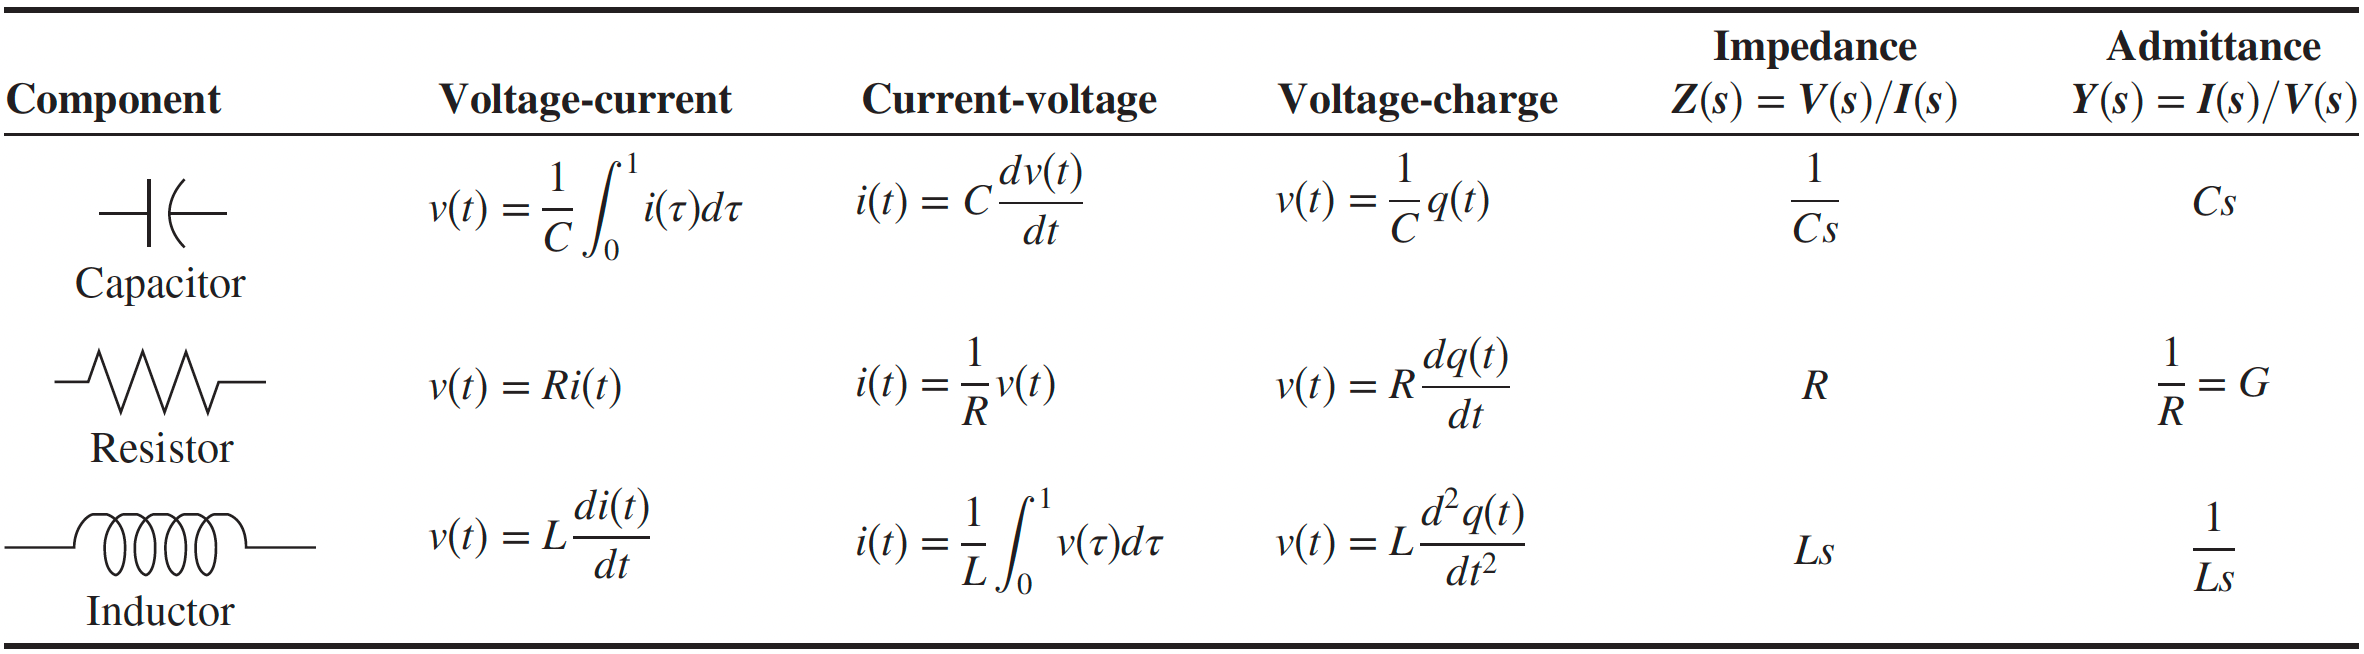
\includegraphics[scale=0.35]{Voltage-Current Table For Transfer Functions}
	\centering
	\caption{Common Electrical Components and Their Transfer Functions}
\end{figure}

The most useful colums are the last two, the rest are just for reference. One important thing to note is that you will use impedence for mesh analysis and admittance for nodal analysis. Impedence is the reciprocal of admittance, and admittance is the reciprocal of impedence.

For most problems, you can assume that the system is linear and time-invariant. This means that the system has zero initial conditions and that the output of the system is directly proportional to the input. Before we start we can use the following properties from \hyperref[fig:Table For Transfer Functions of Electrical Systems]{this table} to our advantage:\\\\

For a capacitor:
\begin{equation}
    V(s)=\frac1{Cs}I(s)
\end{equation}

For a resistor:
\begin{equation}
	V(s)=RI(s)
\end{equation}

For an inductor:
\begin{equation}
	V(s)=LsI(s)
\end{equation}

Defining the transfer function as $Z(s)$:
\begin{equation}
	Z(s)=\frac{V(s)}{I(s)}
\end{equation}

If we have an RLC circuit with one loop (that is, a circuit with one resistor, one inductor, and one capacitor), we can find the transfer function by putting it into the following form:

\begin{equation}
	(\text{Sum of all impedences in the loop}) I(s) = (\text{Sum of applied voltages in the loop})
\end{equation}

Your steps for something like this would be:
\begin{enumerate}
	\item Draw the same circuit, but convert all components into their impedance form.
	\item Factor out the common terms on both sides of the equation
	\item Put it into a form where the output is on the numerator and the input is on the denominator
	\item You now have the transfer function of the system.
\end{enumerate}

Here is an example to help you understand how to find the transfer function of an electrical system:

\begin{problem}[Transfer Function of an RLC Circuit]
Find the transfer function, that is, $Y(s) = I(s)/V(s)$ of the following RLC circuit:
\begin{figure}[H]
	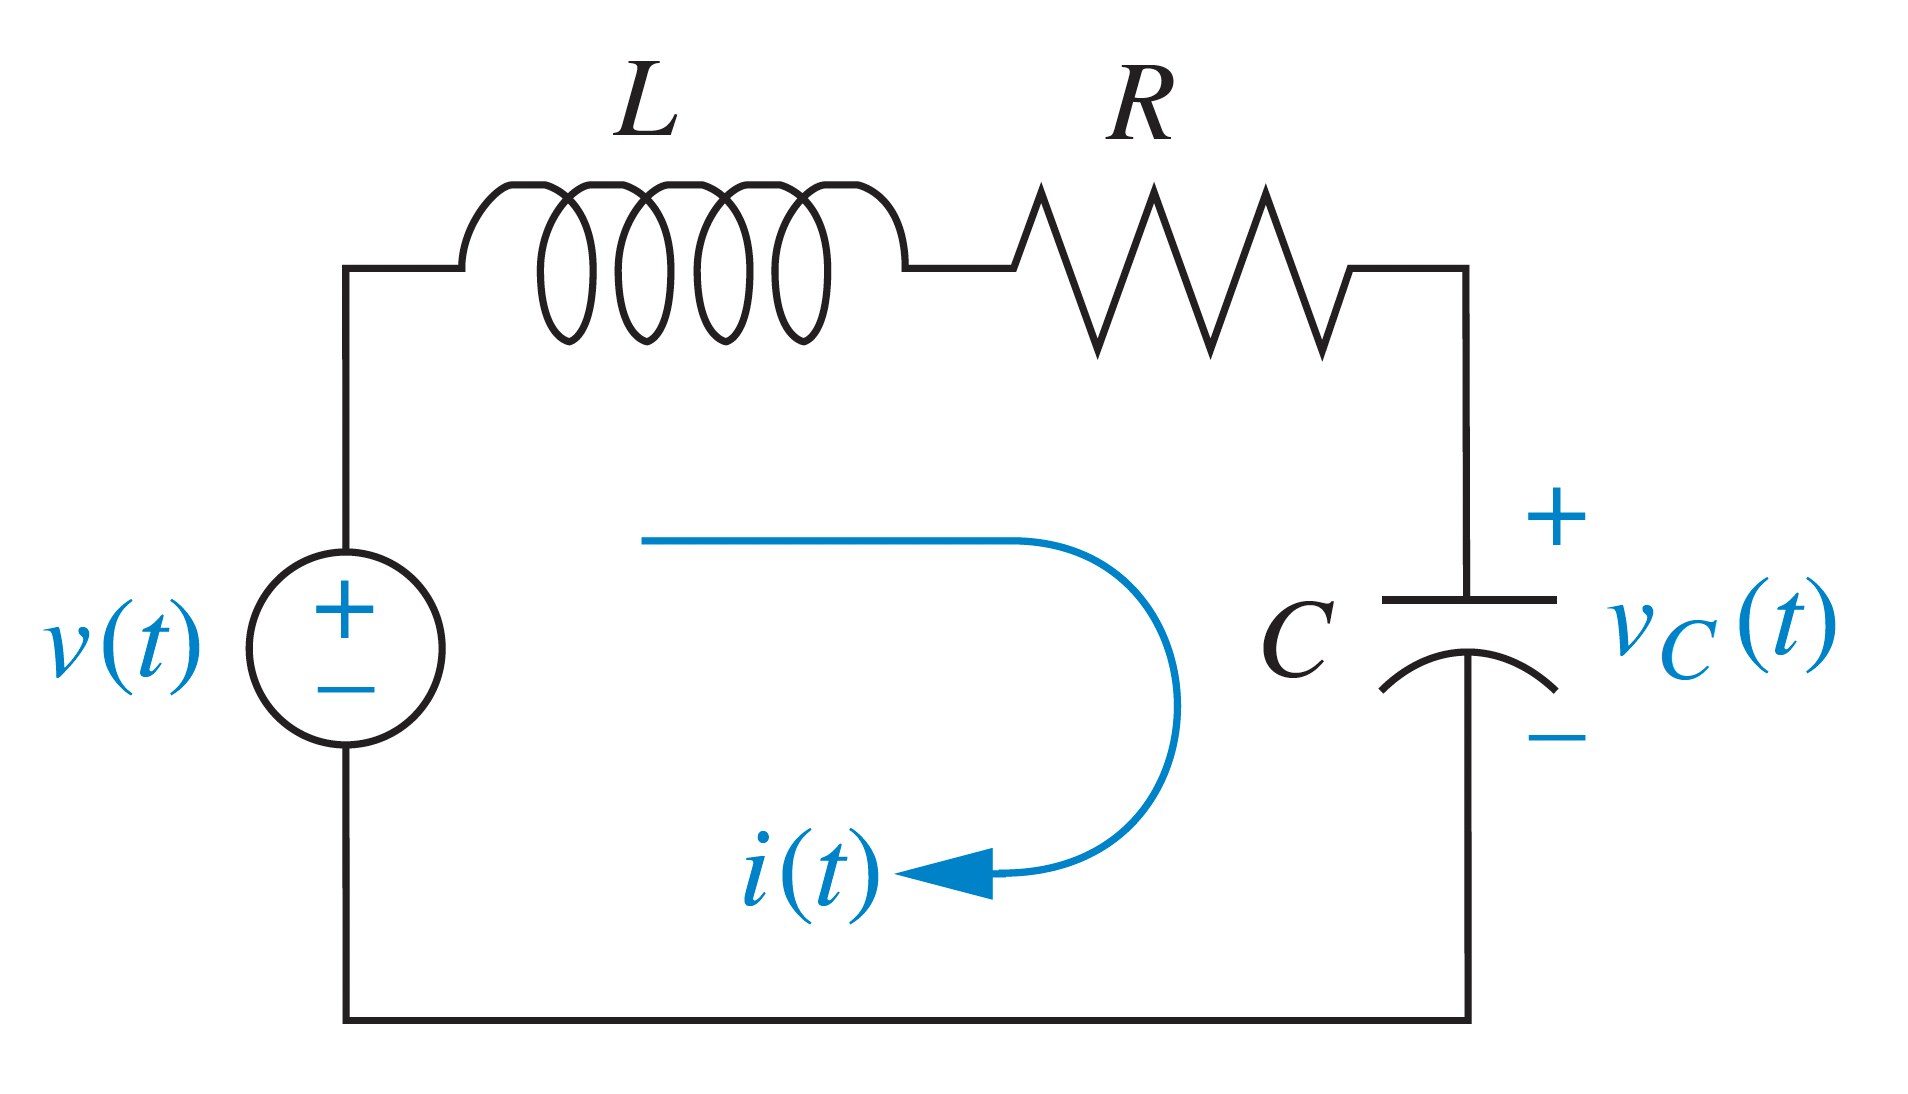
\includegraphics[scale=0.1]{Simple RLC Circuit}
	\centering
	\caption{RLC Circuit}
\end{figure}
\end{problem}



Let's walk through this problem using the steps I outlined above:

\begin{solution}[\textcolor{blue}{Transfer Function of an RLC Circuit}]~
	\begin{enumerate}
		\item Draw the same circuit, but convert all components into their impedance form:
		      \begin{figure}[H]
			      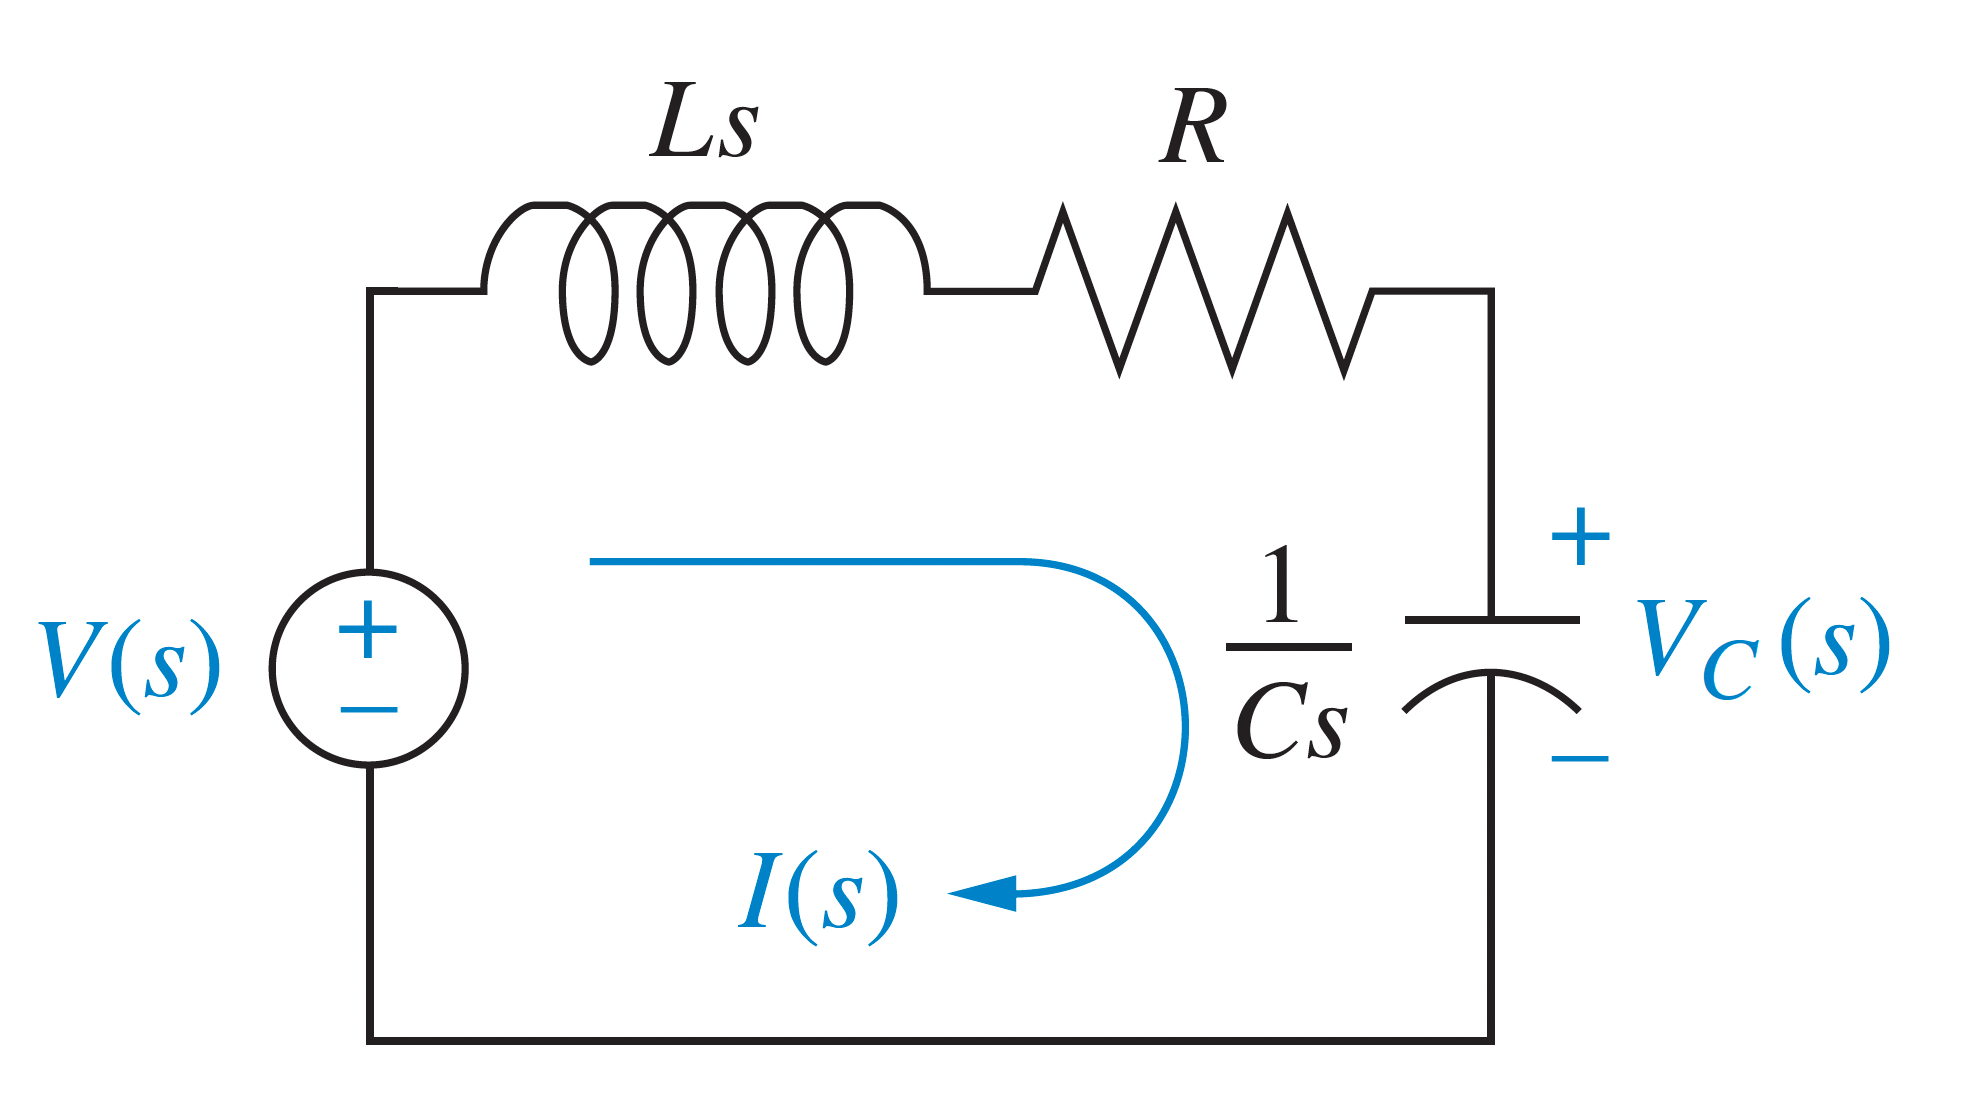
\includegraphics[scale=0.2]{Simple RLC Circuit in Impedence Form}
			      \centering
			      \caption{RLC Circuit in Impedance Form}
		      \end{figure}
		\item Sum up the sides as shown below:
			\begin{equation}
				(\text{Sum of all impedences in the loop}) I(s) = (\text{Sum of applied voltages in the loop})
			\end{equation}
		Therefore, the equation becomes:
			\begin{equation}
			      (Ls + R + \frac{1}{Cs})I(s) = V(s)
		      \end{equation}
		\item Put it into a form where the output is on the numerator and the input is on the denominator:
		      \begin{equation}
			      \frac{I(s)}{V(s)} = \frac{1}{Ls + R + \frac{1}{Cs}}
		      \end{equation}
	\end{enumerate}
\end{solution}

This isn't what you would usually be asked, you would usually be asked something like:
\begin{problem}[Transfer Function of an RLC Circuit - Cont.]
Find the transfer function of the following RLC circuit that relates the capacitor voltage, $V_c(s)$, to the input voltage, $V(s)$:
\begin{figure}[H]
	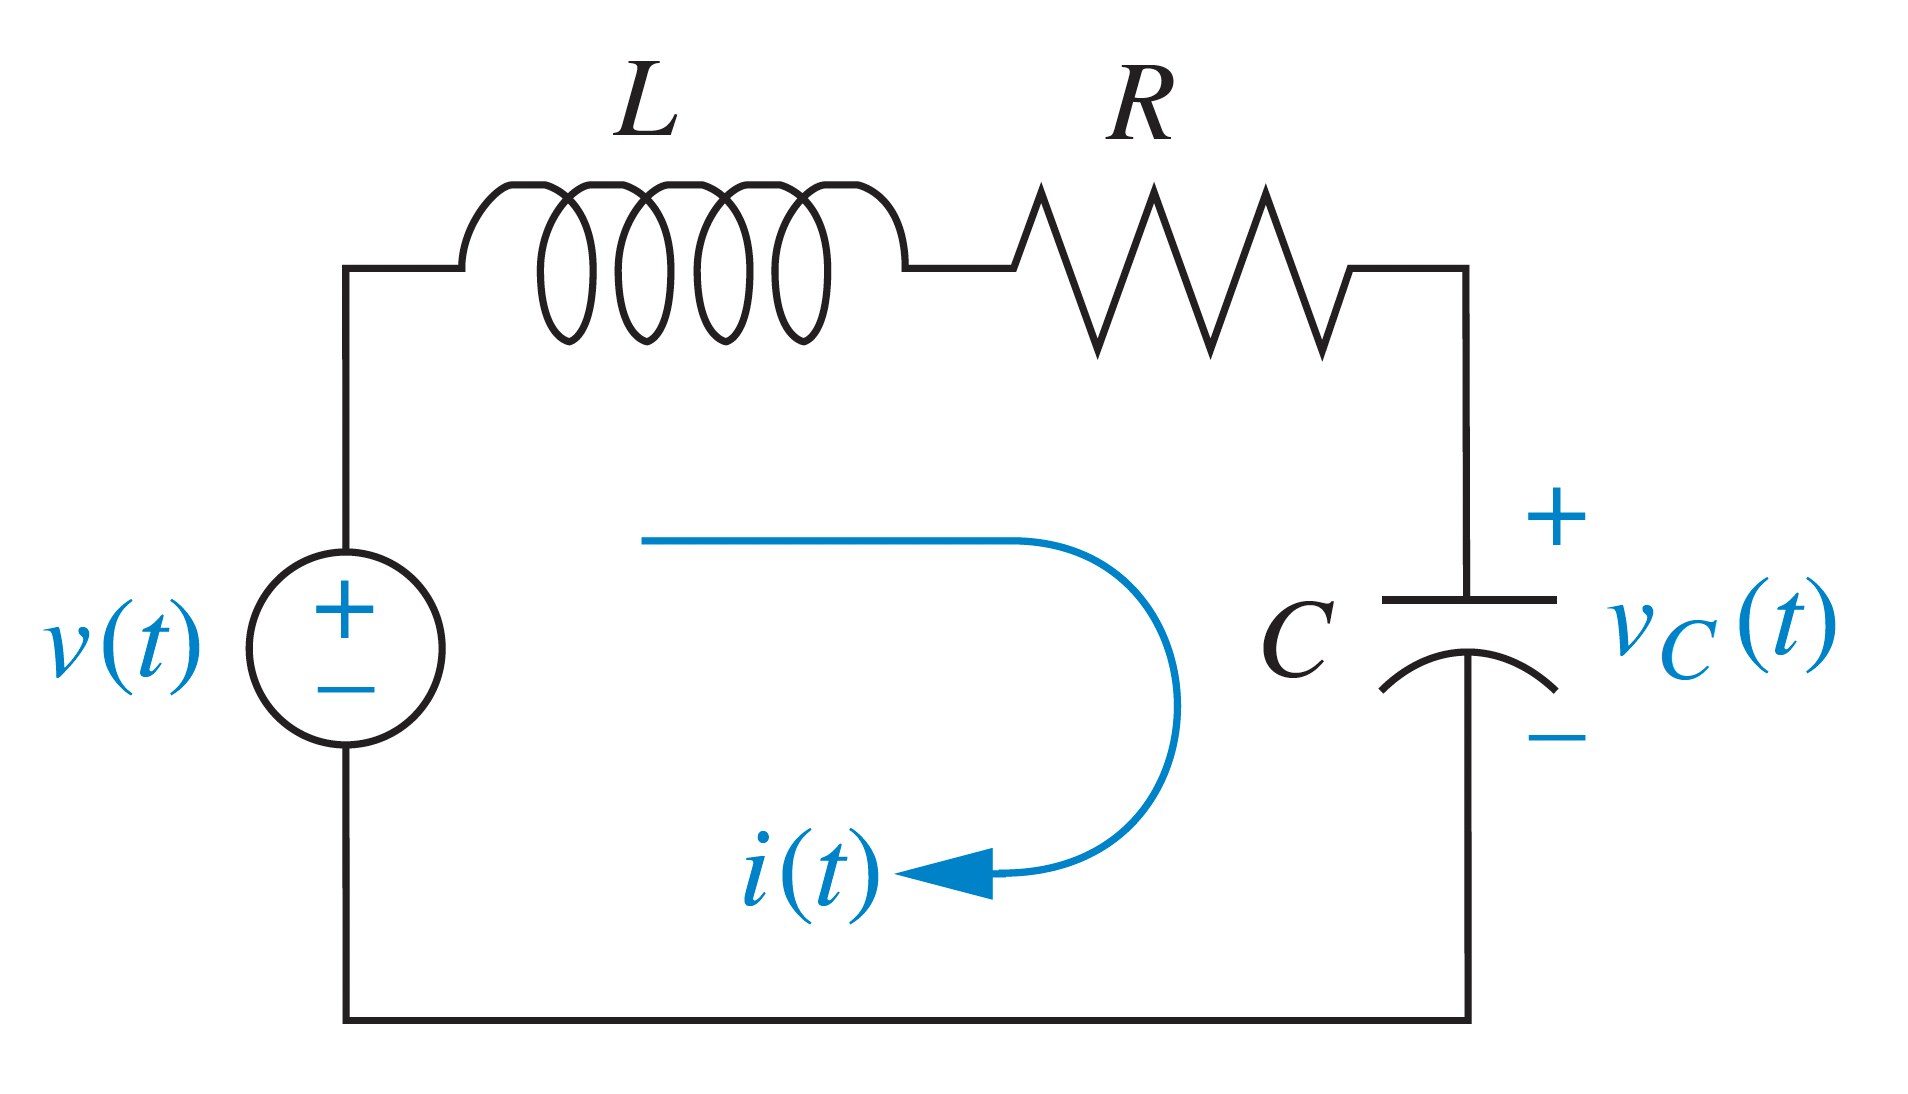
\includegraphics[scale=0.1]{Simple RLC Circuit}
	\centering
	\caption{RLC Circuit}
\end{figure}
\end{problem}

\begin{solution}[\textcolor{blue}{Transfer Function of an RLC Circuit - Cont.}]~
	\\We got most of the way there with the previous steps. For your reference, the input voltage $V(s)$ is:
	\begin{equation}
		V(s) = (Ls + R + \frac{1}{Cs})I(s)
	\end{equation}
	And the circuit is:
	\begin{figure}[H]
		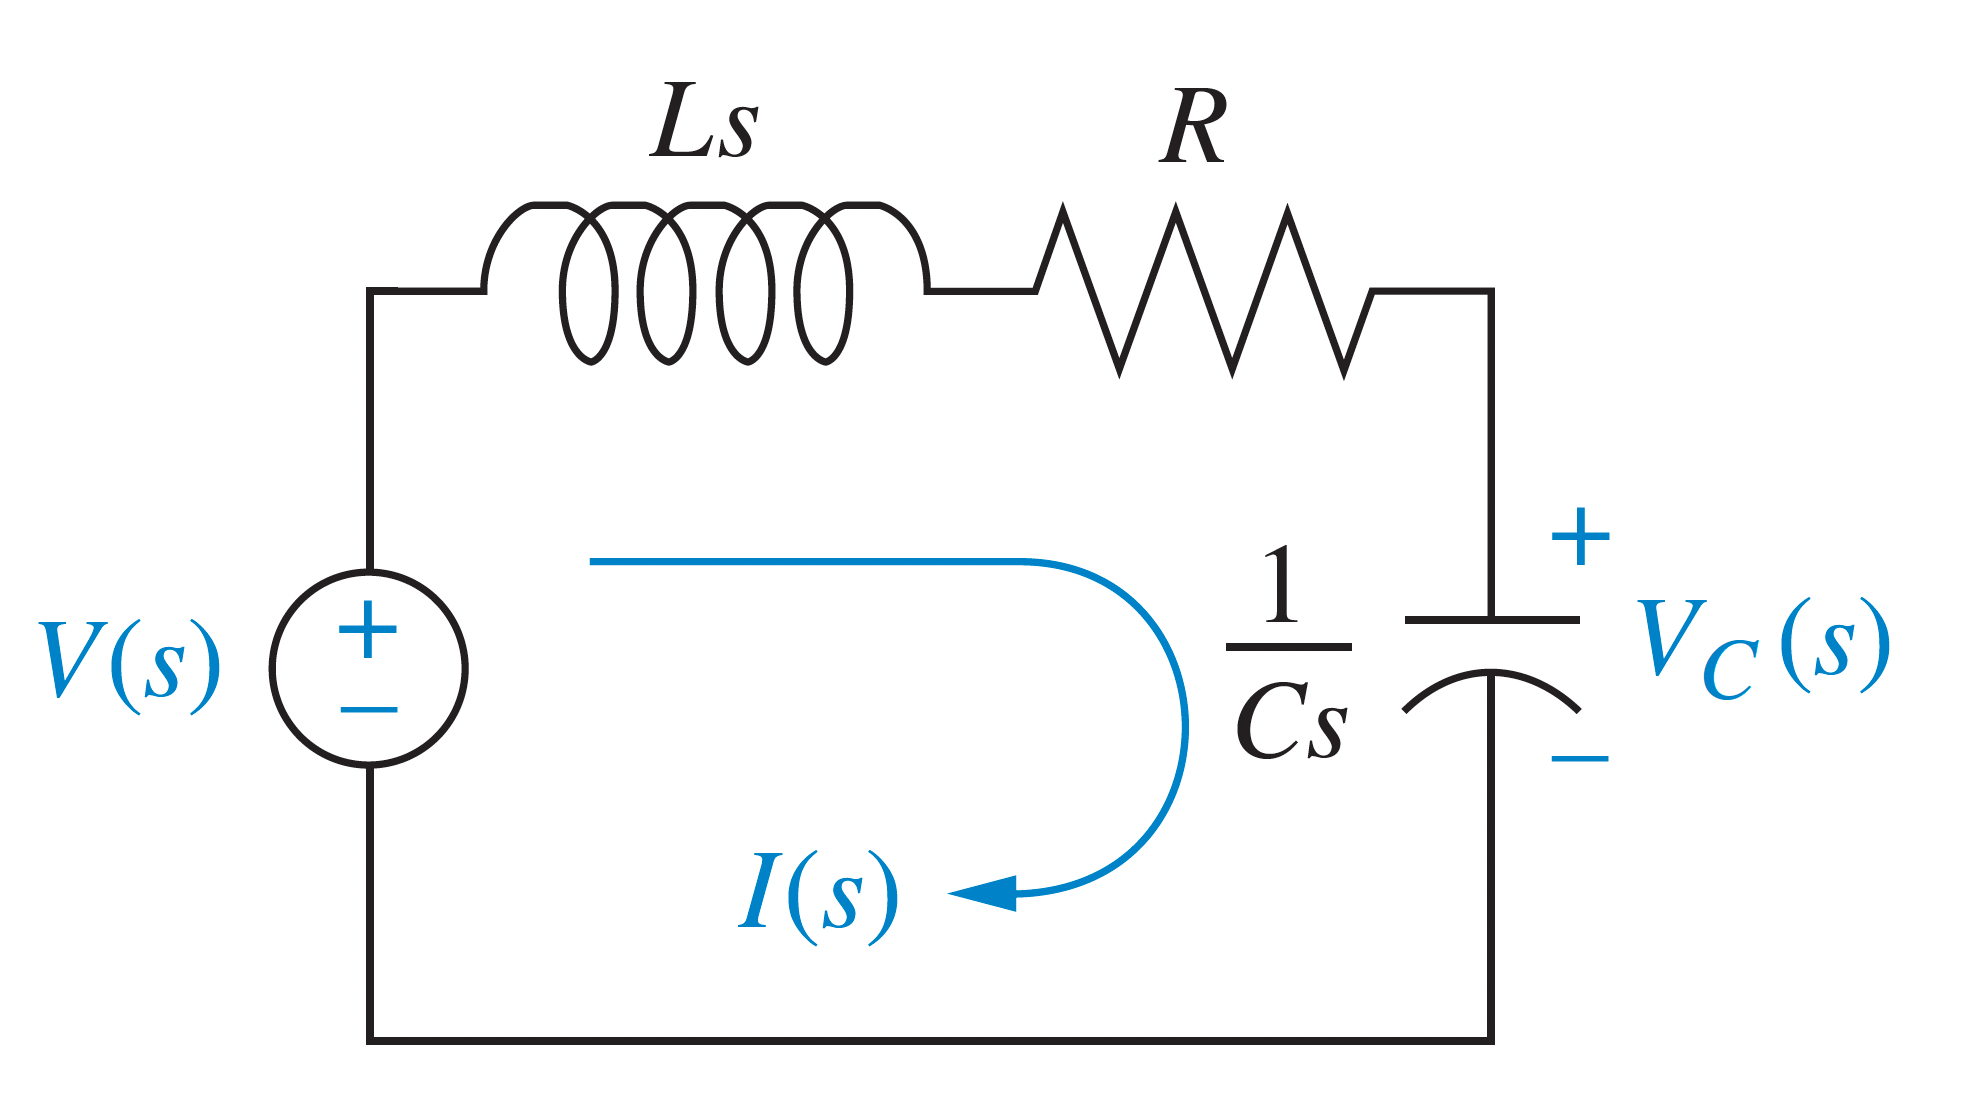
\includegraphics[scale=0.2]{Simple RLC Circuit in Impedence Form}
		\centering
		\caption{RLC Circuit in Impedance Form}
	\end{figure}
\begin{enumerate}
	\item Since we know that:
	\begin{equation}
		V_c(s) = \frac{1}{Cs}I(s)
	\end{equation}
	Which means:
	\begin{equation}
		V_c(s) Cs =I(s)
	\end{equation}
	\item We can substitute $V_c(s)$ with the transfer function we found in the previous problem:
	\begin{equation}
		V(s) = (Ls + R + \frac{1}{Cs})I(s) = (Ls + R + \frac{1}{Cs})(Cs)V_c(s) 
	\end{equation}
	\begin{equation}
		V(s) = (L C s^{2} + R C s + 1) V_{c}{(s)}
	\end{equation}
	This means:
	\begin{equation}
		\frac{V_c(s)}{V(s)} = \frac{1}{L C s^{2} + R C s + 1}
	\end{equation}
	\item We can simplify this to:
	\begin{equation}
		\frac{V_c(s)}{V(s)} =\frac{\frac{1}{LC}}{s^2 + \frac{R}{L}s + \frac{1}{LC}}
	\end{equation}
	This form is the transfer function of the system that can easily be put into a partial fraction that you can take the inverse laplace of.
	\end{enumerate}
\end{solution}

Realistically, you won't be asked a question like this on a test, but this question is a base for understanding the next problem, whcih is more akin to what may be on a test. Let's talk about another scenario you may encounter, where there are now 2 loops. This is a bit more complex, but the steps are very similar:

\begin{enumerate}
	\item Draw the same circuit, but convert all components into their impedance form.
	\item Sum up the impedences like you did before, but now you will have two equations. One for each loop. It will look something like this:
	\begin{equation}
		\left.\left[\begin{array}{c}\text{Sum of}\\\text{impedances}\\\text{around Mesh 1}\end{array}\right.\right]I_1(s)-\left[\begin{array}{c}\text{Sum of}\\\text{impedances}\\\text{common to the}\\\text{two meshes}\end{array}\right]I_2(s)=\left[\begin{array}{c}\text{Sum of applied}\\\text{voltages around}\\\text{Mesh 1}\end{array}\right]
	\end{equation}
	\begin{equation}
		-\begin{bmatrix}\text{Sum of}\\\text{impedances}\\\text{common to the}\\\text{two meshes}\end{bmatrix}I_1(s)+\begin{bmatrix}\text{Sum of}\\\text{impedances}\\\text{around Mesh}2\end{bmatrix}I_2(s)=\begin{bmatrix}\text{Sum of applied}\\\text{voltages around}\\\text{Mesh}2\end{bmatrix}
	\end{equation}
	\item Use \hyperref[subsec:Cramers_Rule]{Cramer's Rule} to solve for either $I_1(s)$ or $I_2(s)$, depending on what you are asked for.
	\item Put it into a form where the output is on the numerator and the input is on the denominator.
	\item You now have the transfer function of the system.
\end{enumerate}


%%%%%%%%%%%%%%%%%%%%%%%%%%% End of Document %%%%%%%%%%%%%%%%%%%%%%%%%%%%%%%
\end{document}